\chapter{Caches}
\section{Why Caches}
The difference between cycle time (time of a stage in a pipeline) and memory access time has continually increased.
\begin{center}
    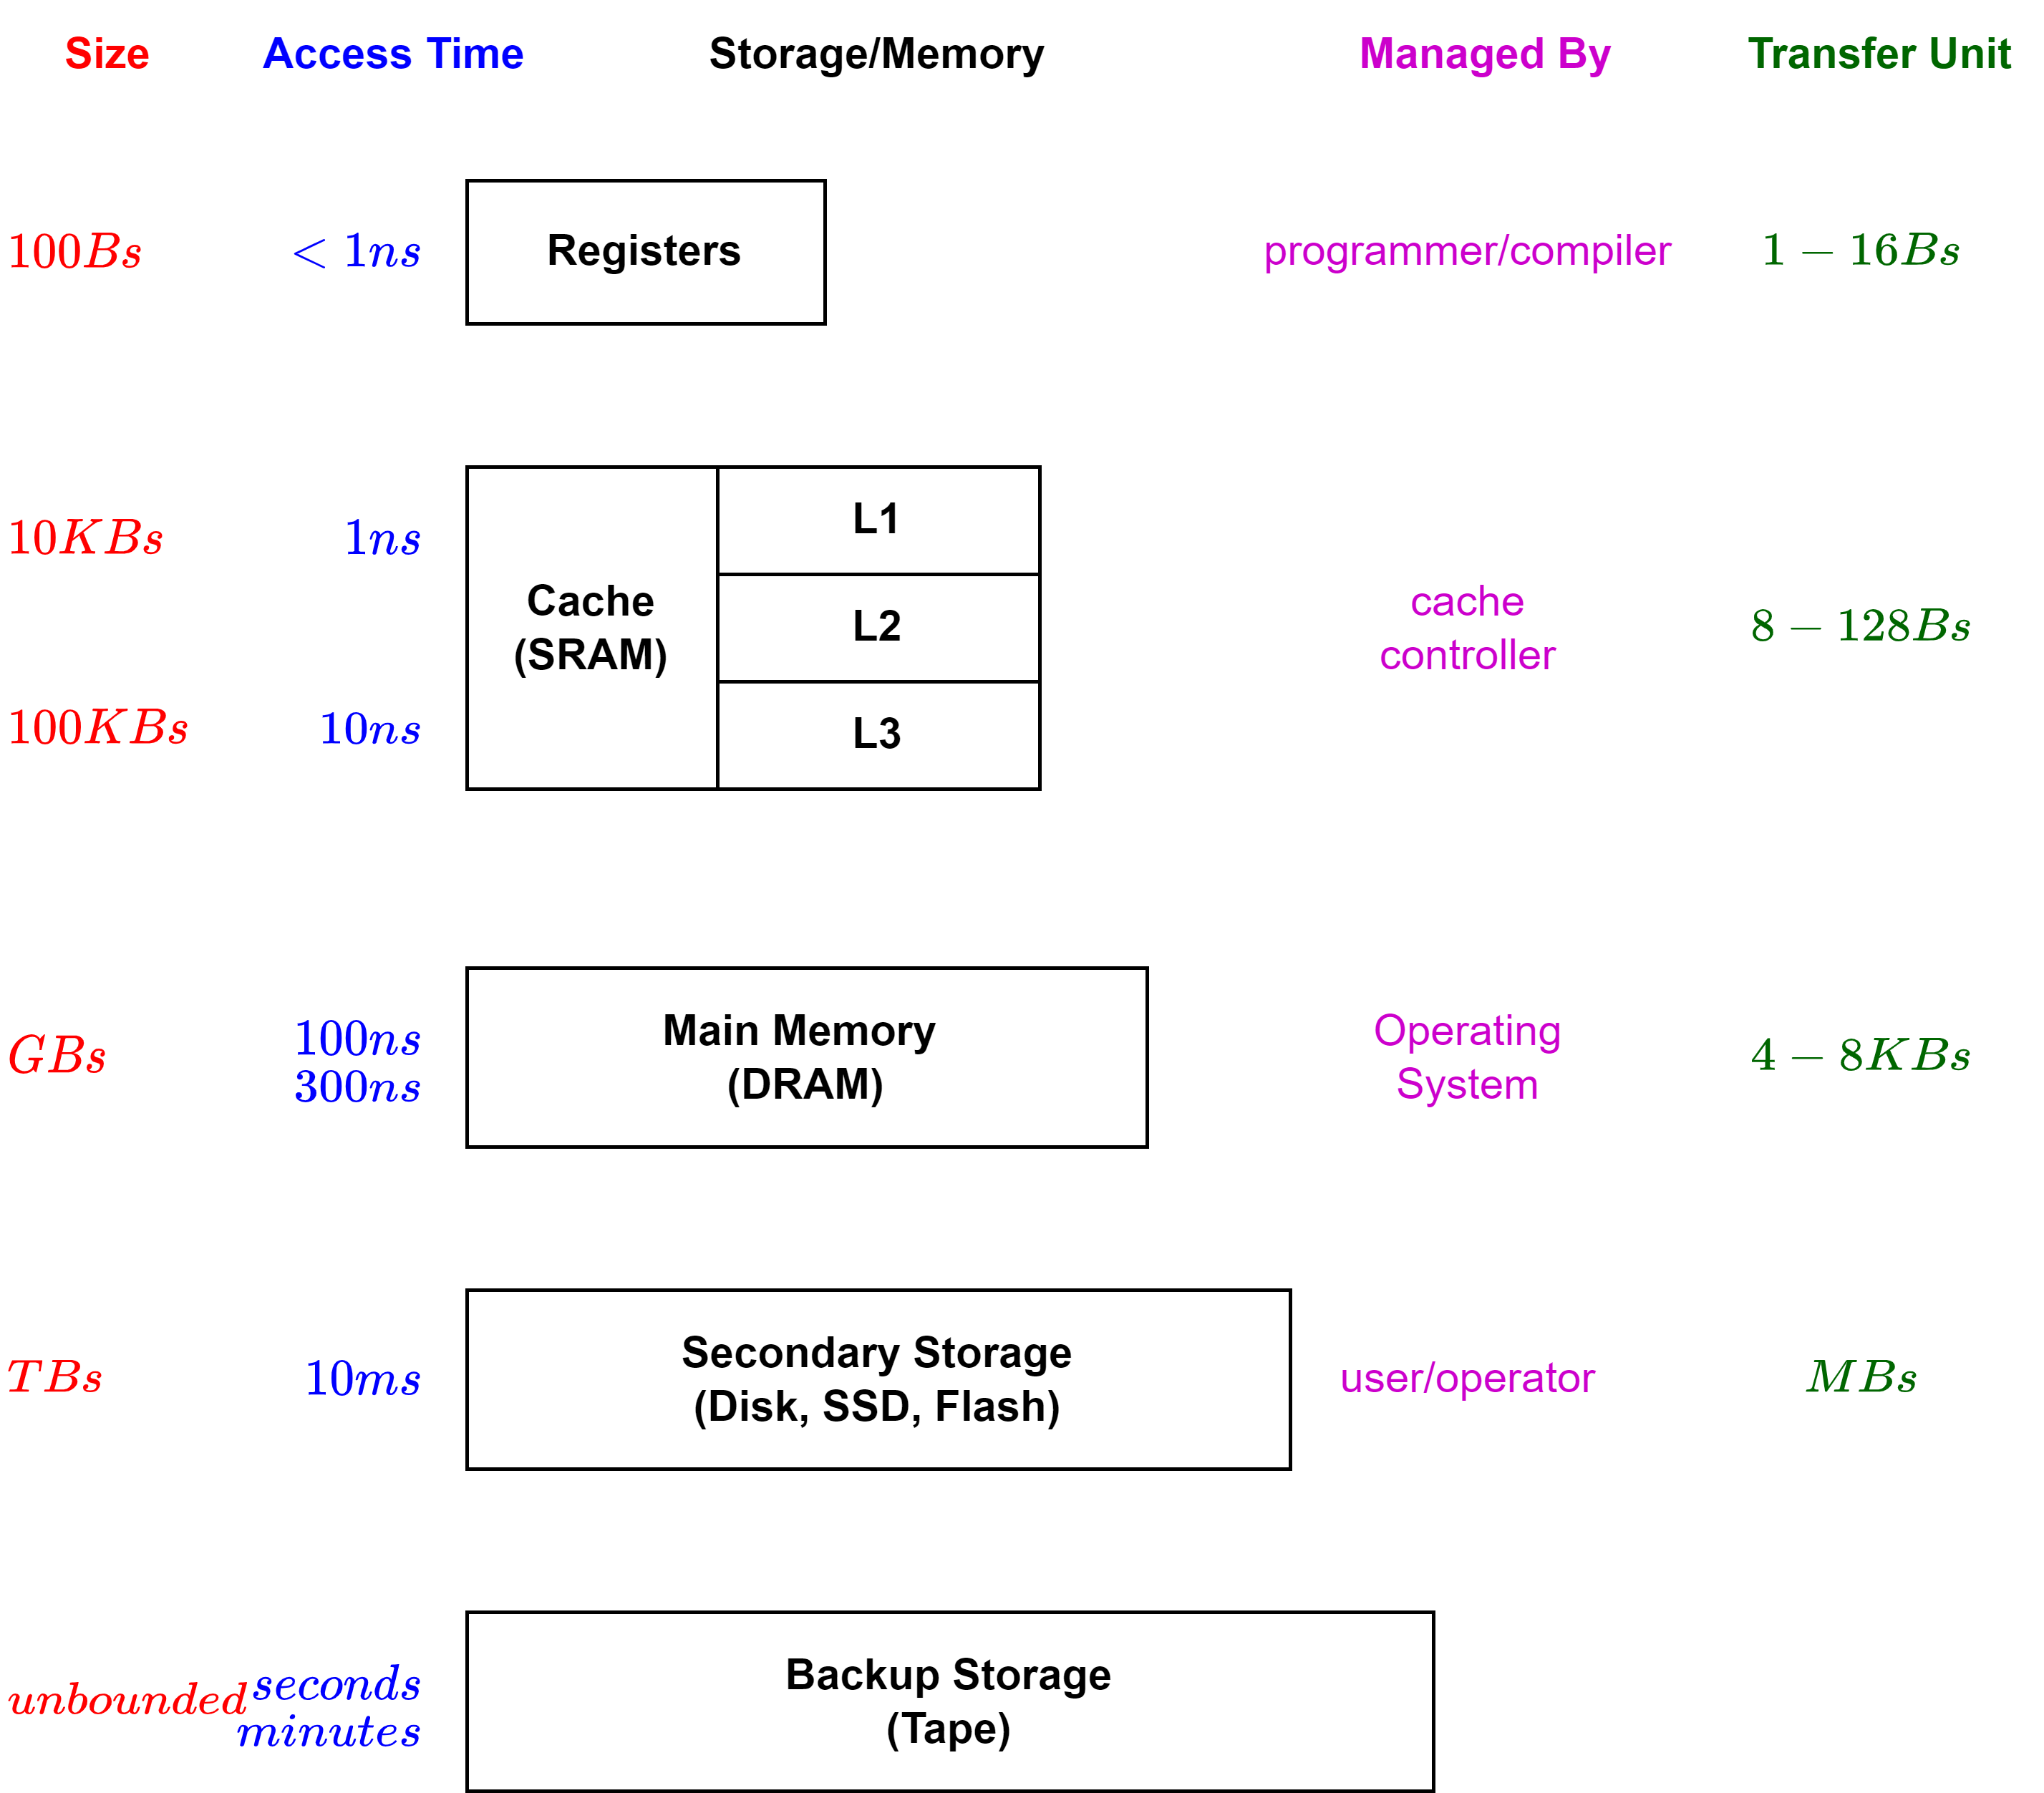
\includegraphics[width=.9\textwidth]{caches/images/memory_hierarchy.drawio.png}
\end{center}
\section{Locality}
Programs typically access only a small part of their address space during a short time period.
\begin{tcbraster}[raster columns=2,raster equal height]
    \begin{definitionbox}{Temporal Locality}
        Locality in time. The same location referenced is often referenced multiple times.
    \end{definitionbox}
    \begin{definitionbox}{Temporal Locality}
        Locality in space. Locations near an accessed location tend to be referenced soon.
    \end{definitionbox}
\end{tcbraster}
Most modern architectures are reliant on locality to determine when and what locations should be cached.
\begin{itemize}
    \item Cache is a scarce resource.
    \item Cache misses are expensive.
\end{itemize}

\section{Cache Types}
\subsection{Directly Mapped Cache}
\begin{definitionbox}{Associativity Conflicts}
    Where two or more locations are mapped to the same cache line/set of cache lines, and repeatedly replace each other.
    \begin{minted}{C}
/* Example with arrays, assume cache line is 256 bytes
 * and both arrays start at same cache index 
 */

int array_a[64];
int array_b[64];

int some_function() {
    int sum = 0;
    for (int i = 0; i < 64; i++) {
        r += 
        array_a[i]    /* array_a moved into cache line */
        + array_b[i]; /* array_b evicts array_a and replaces */
    }
    return sum;
}
    \end{minted}
\end{definitionbox}

\begin{center}
    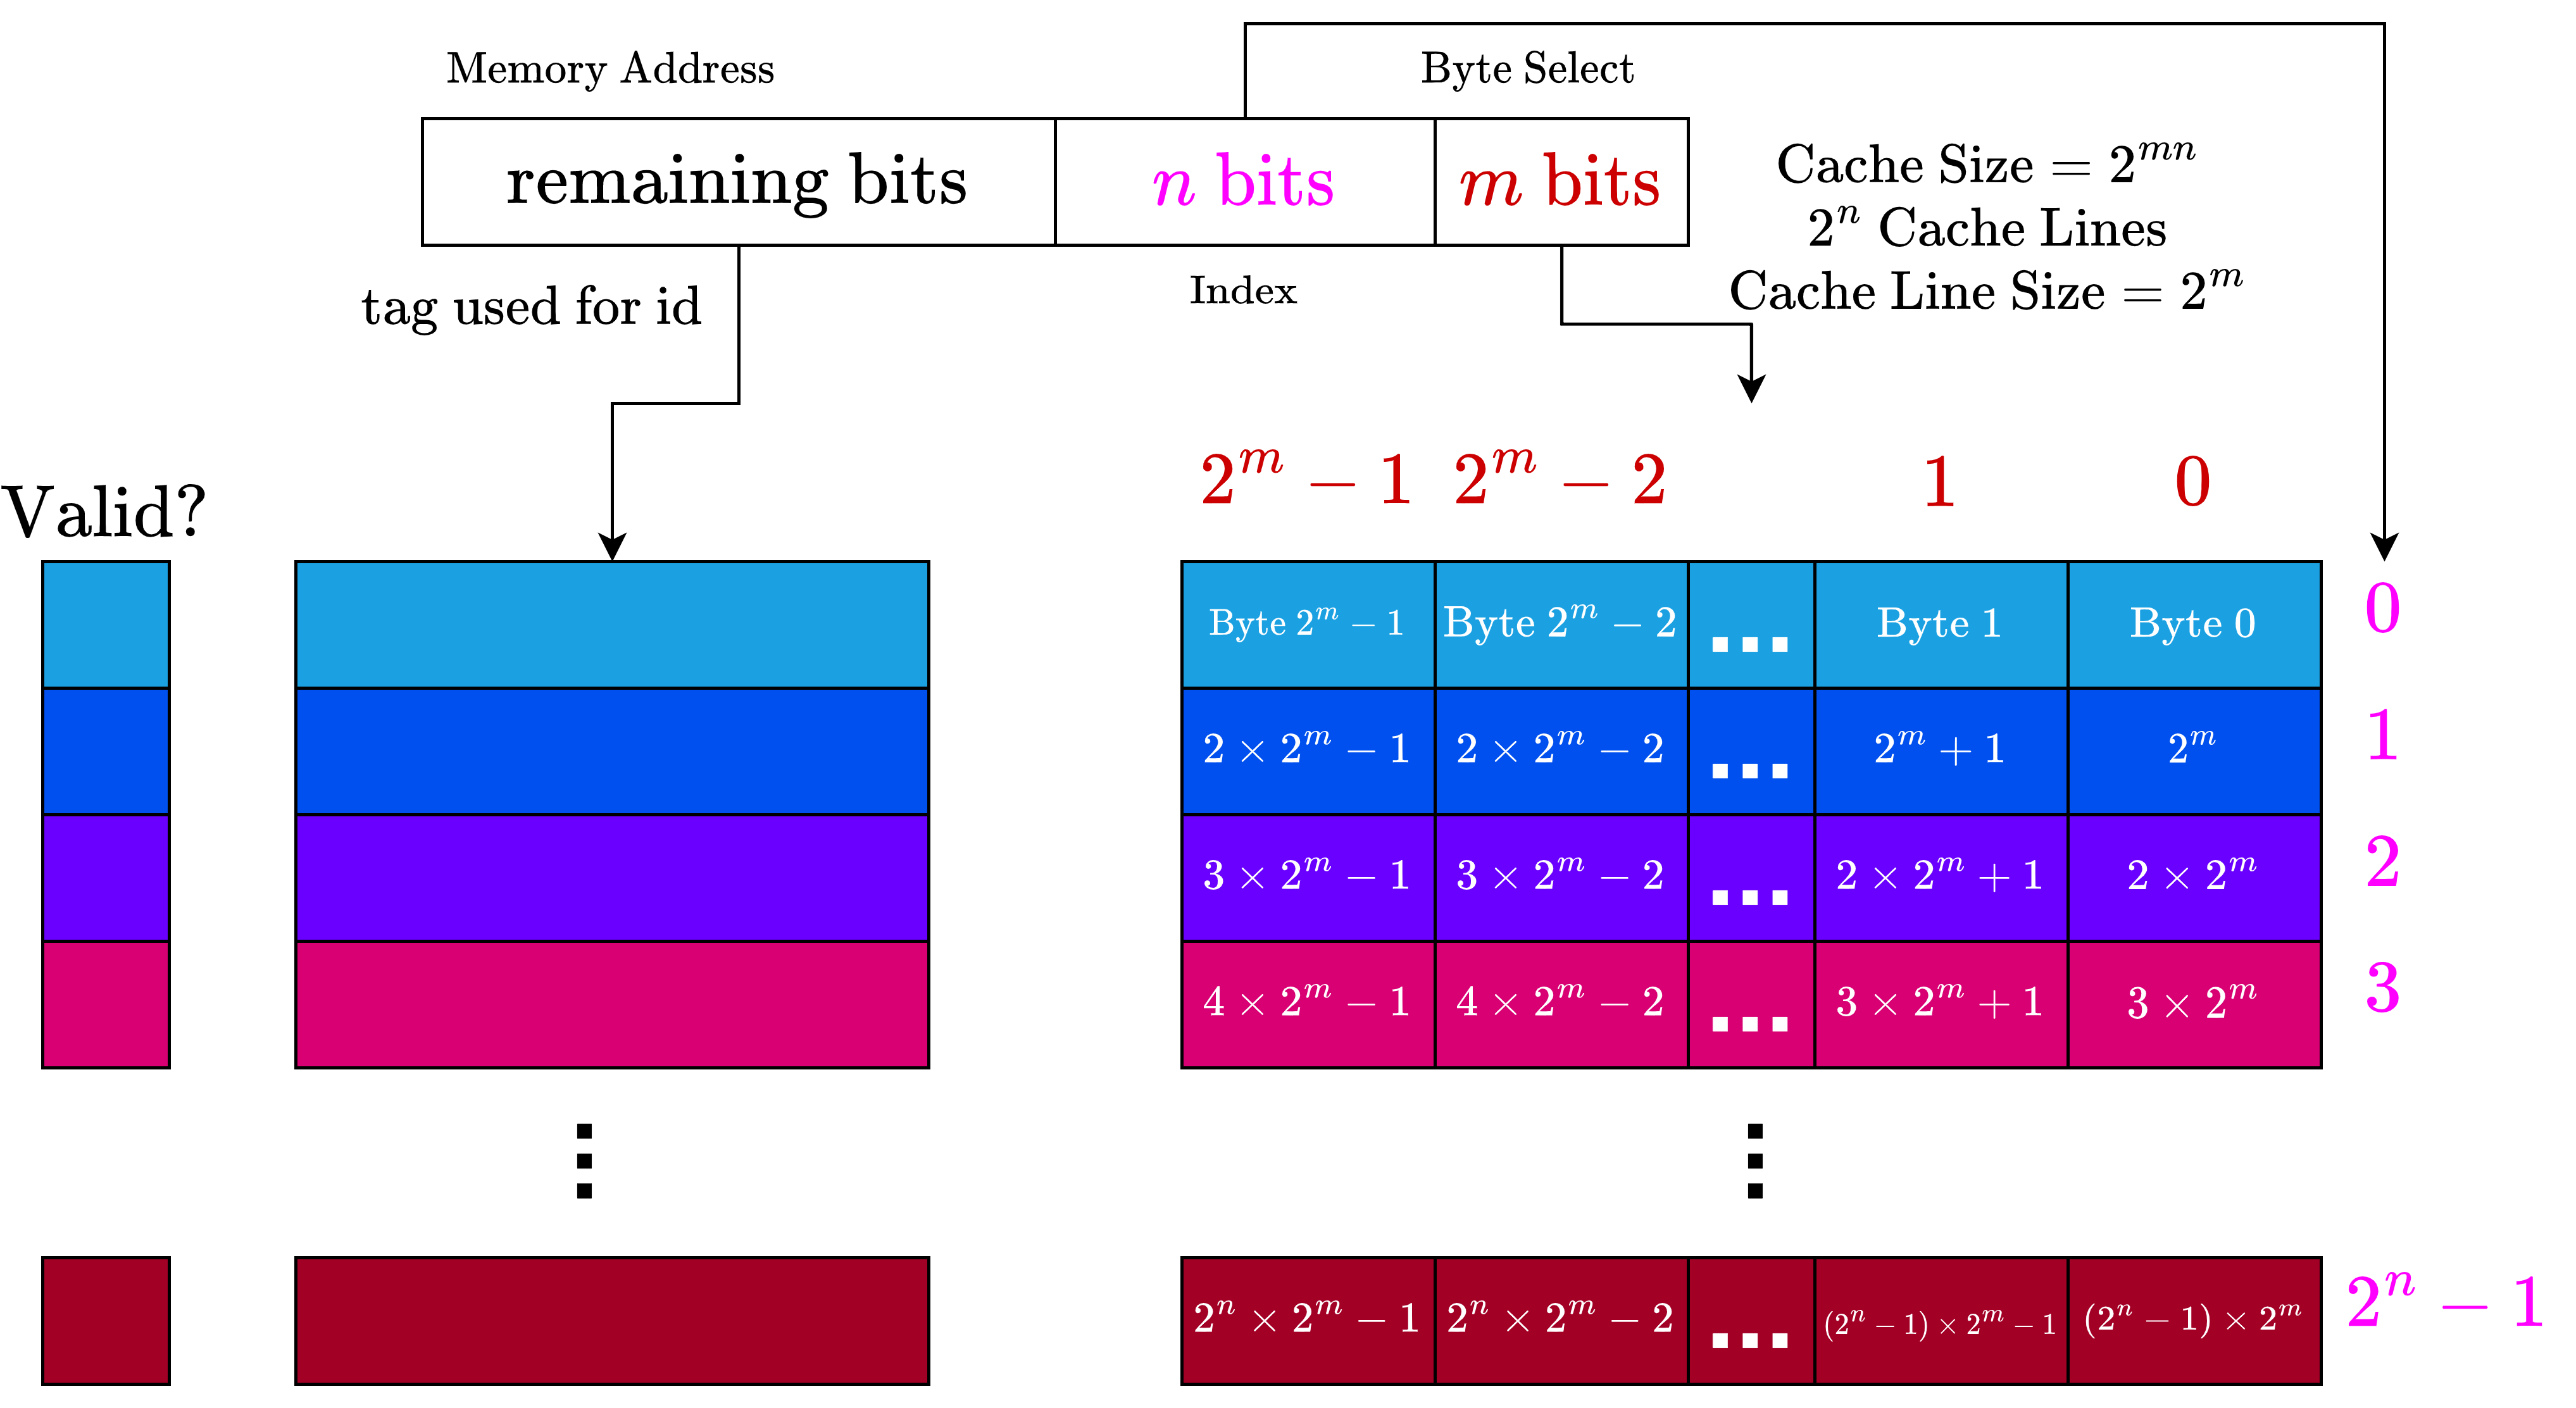
\includegraphics[width=.9\textwidth]{caches/images/direct_mapped_cache.drawio.png}
\end{center}
\begin{itemize}
    \item Index and byte select used to find entry. Then tag compared to determine hit/miss.
    \item We can see a pattern in memory of where locations can be cached based on the index.
    \item Block/line received before the hit/miss is known (recover later if miss).
\end{itemize}
\begin{center}
    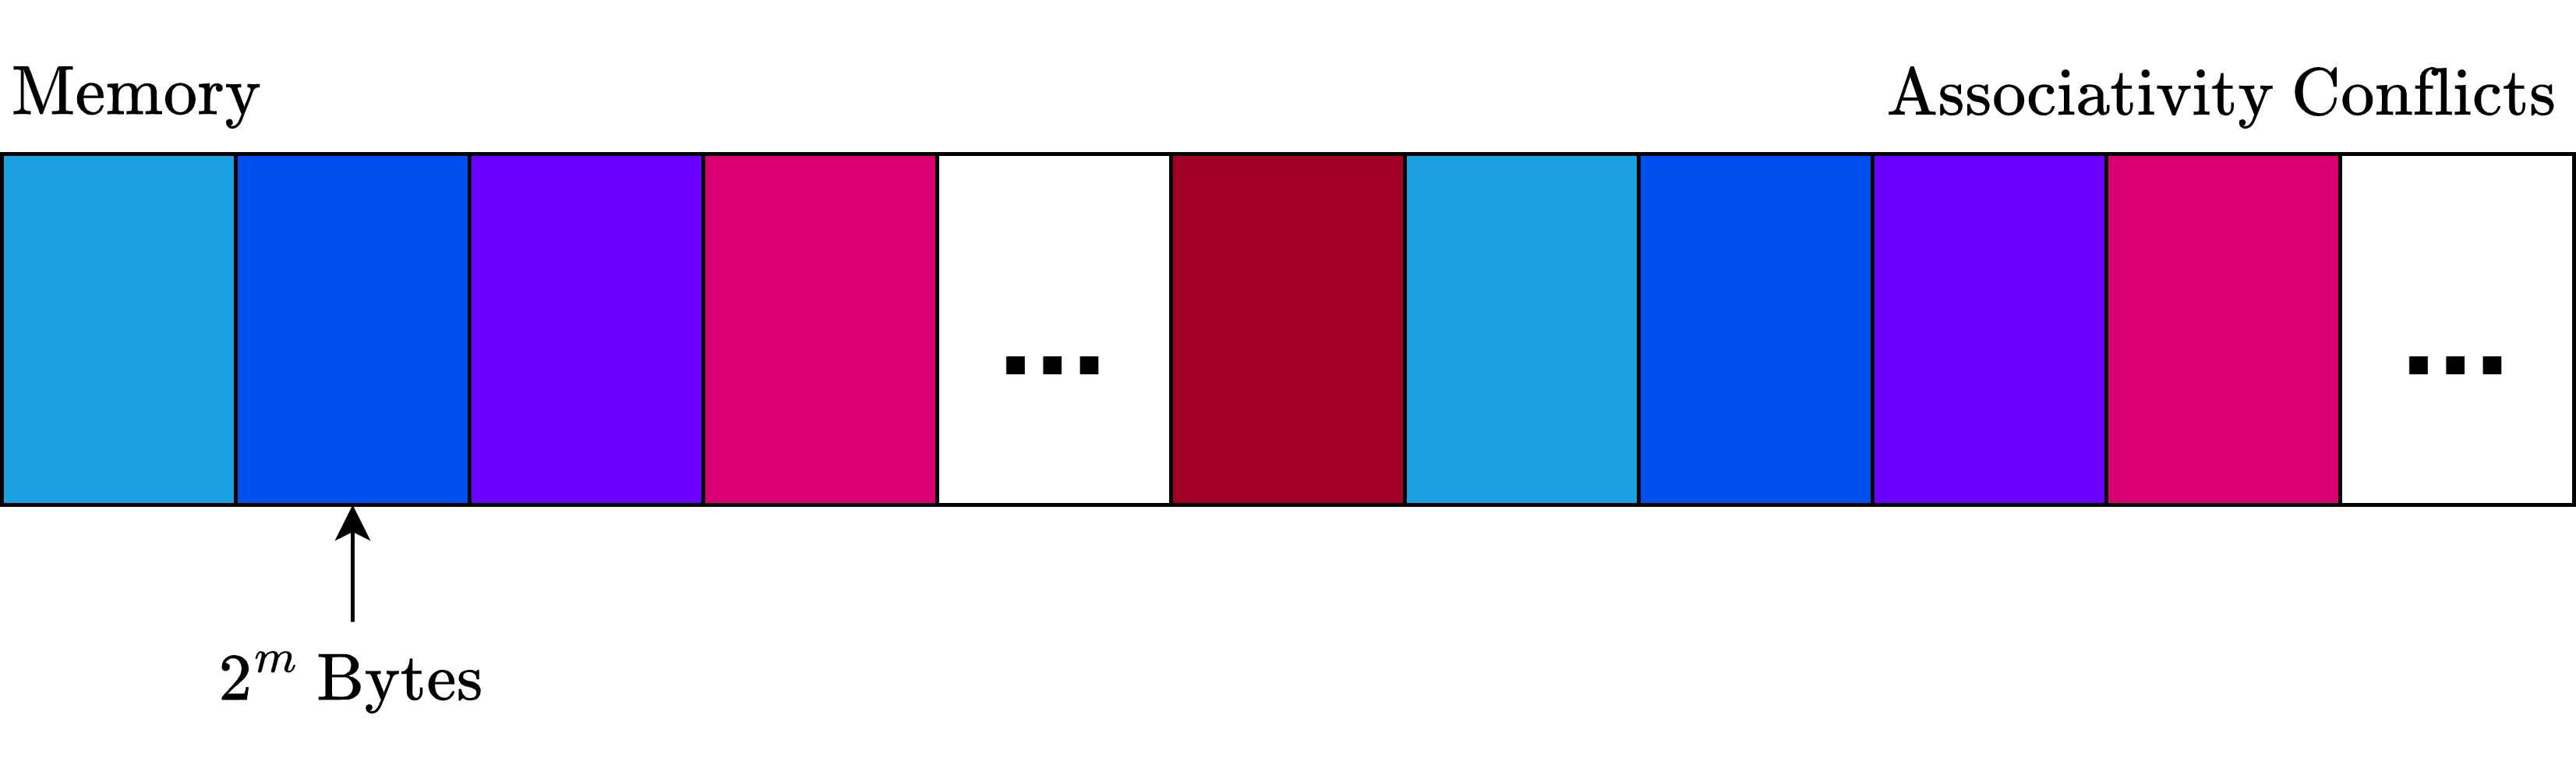
\includegraphics[width=.9\textwidth]{caches/images/associativity_conflicts.drawio.png}
\end{center}
\begin{prosbox}
    \begin{center}
        \begin{tabular}{r p{.8\textwidth}}
            \textbf{Simplicity} & Simple indexing of cache \& compare to determine hit/miss. \\
            \textbf{Fast Lookup} & Only one location where a cached value may be. \\
        \end{tabular}
    \end{center}
\end{prosbox}
\begin{consbox}
    \begin{center}
        \begin{tabular}{r p{.8\textwidth}}
            \textbf{Associativity Conflicts} & As location can only be cached in one place, associativity conflicts are common. \\
        \end{tabular}
    \end{center}
\end{consbox}

\subsection{Two Way Associative}
Combine two directly mapped caches, and only cache a given location in one.
\begin{center}
    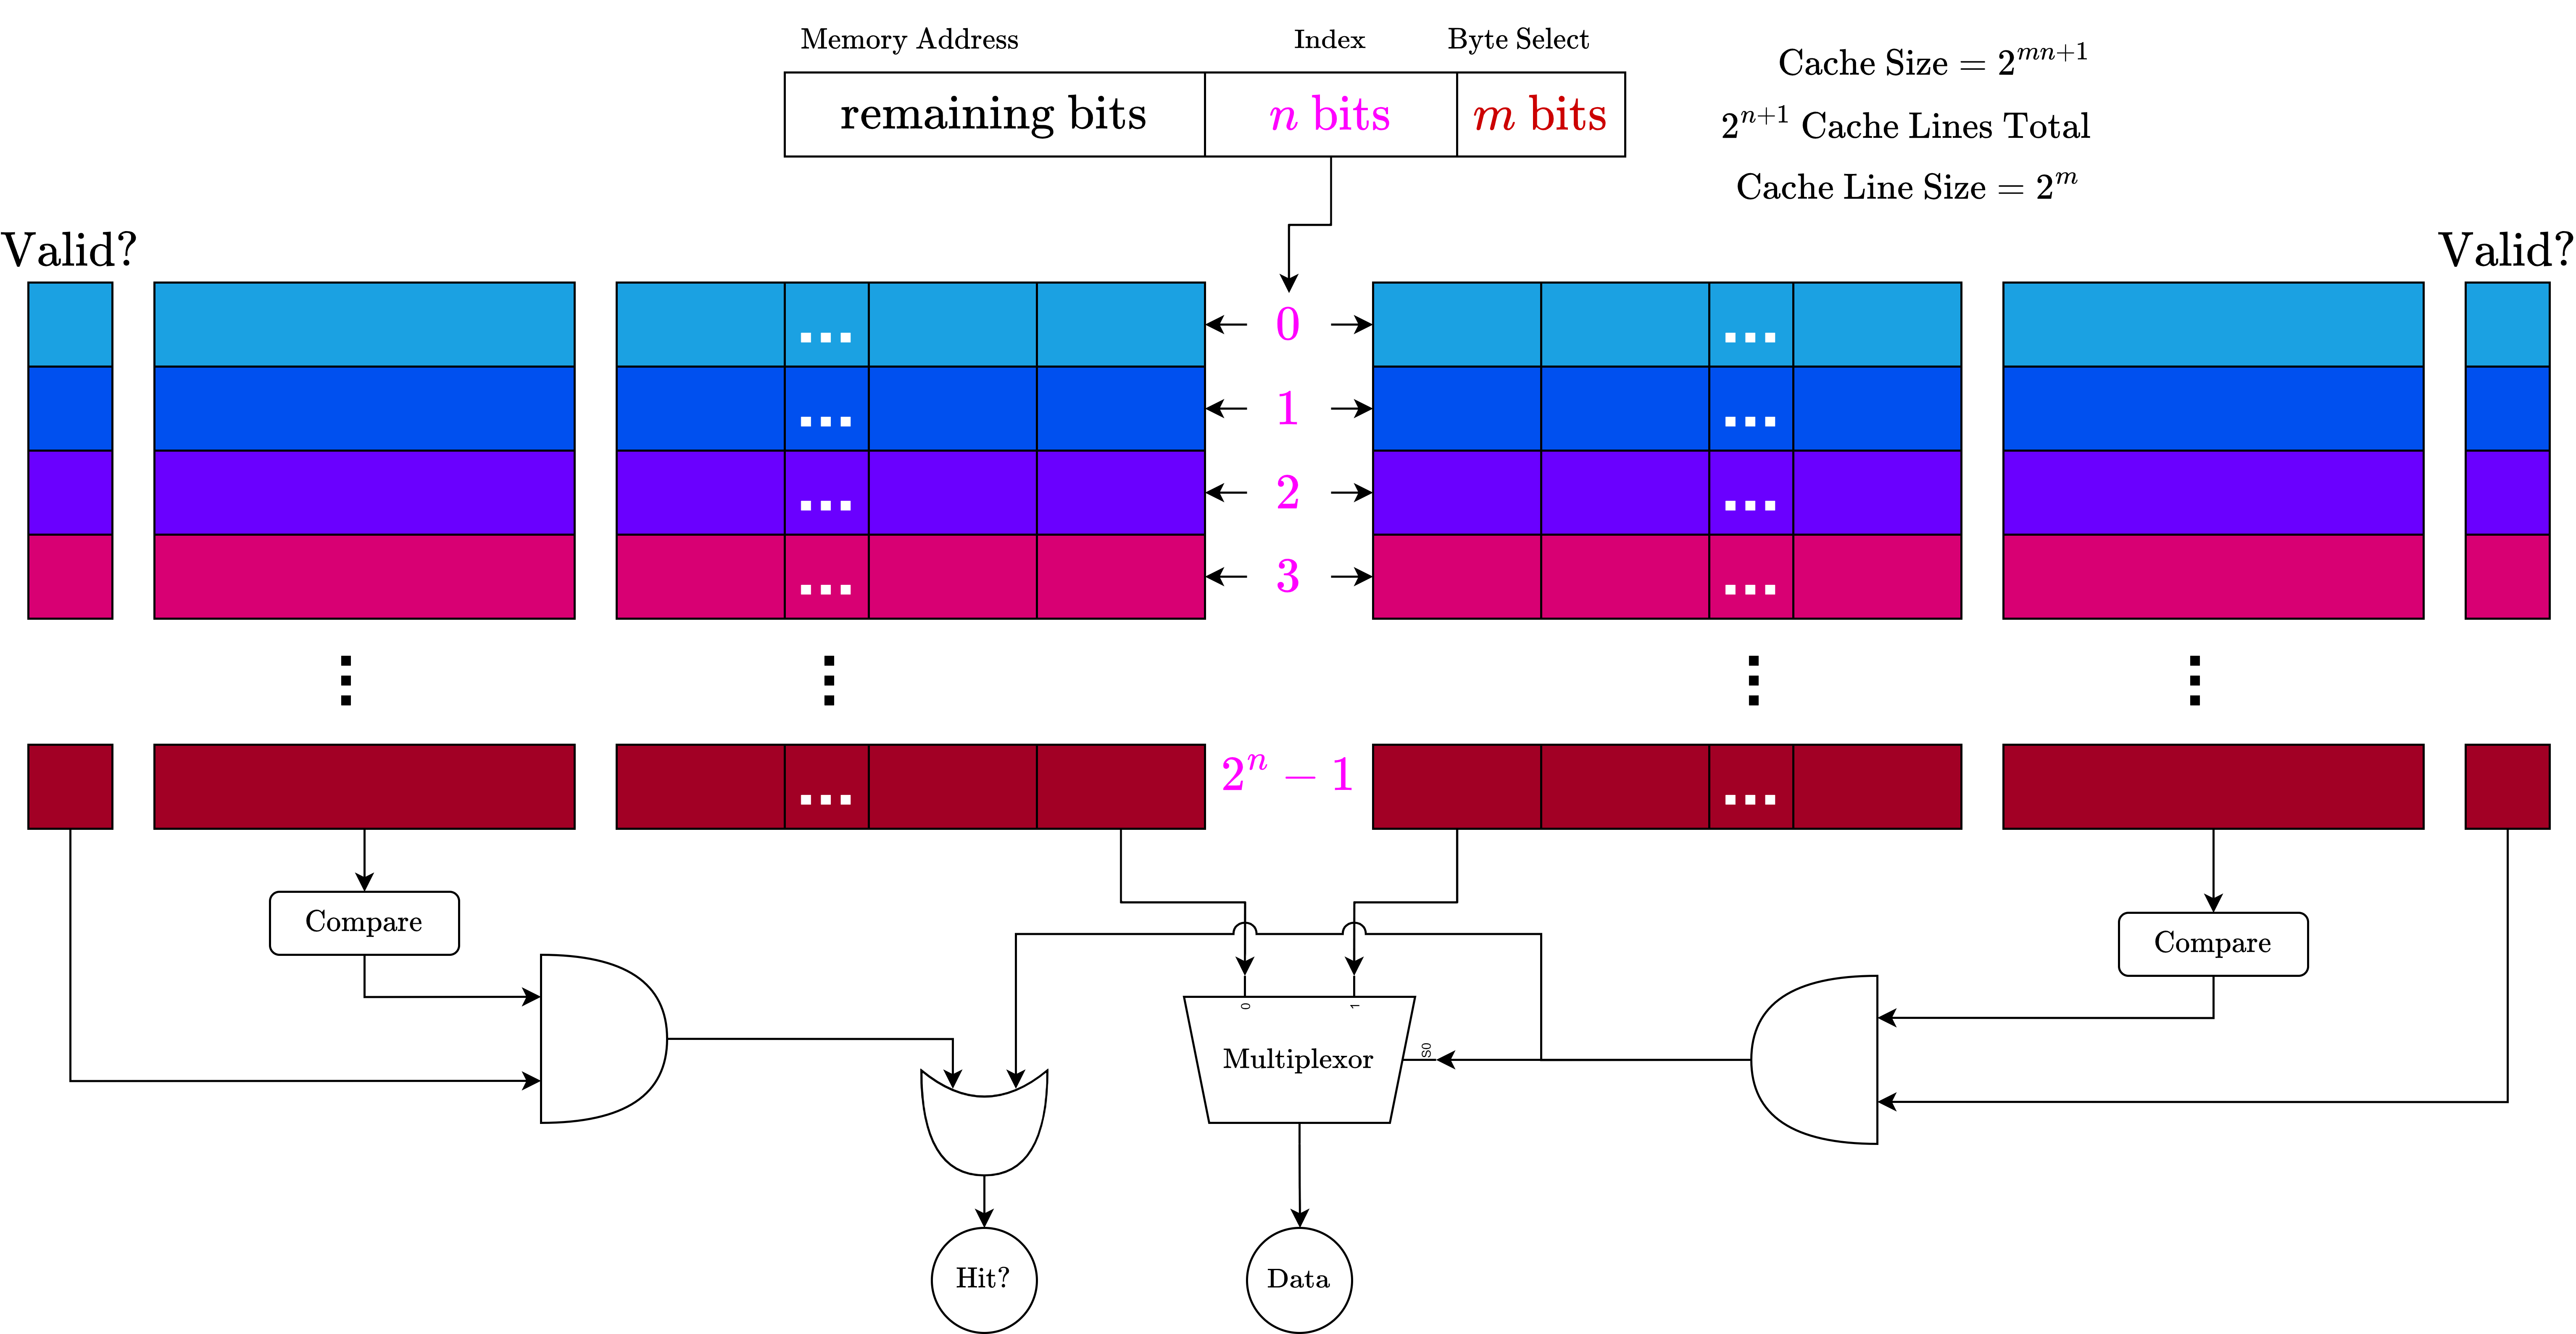
\includegraphics[width=.9\textwidth]{caches/images/two_way_set_associative.drawio.png}
\end{center}
\begin{itemize}
    \item Both caches searched in parallel.
    \item Only one hit possible, this is selected from result of both caches (selection is in the critical path)
    \item Cache block/line is available after the hit/miss is determined.
\end{itemize}

\begin{prosbox}
    \begin{center}
        \begin{tabular}{r p{.8\textwidth}}
            \textbf{Fewer Assoc Conflicts} & Any location can now select two different locations in the cache, hence two addresses with the same index can both be cached. \\
            \textbf{}
        \end{tabular}
    \end{center}
\end{prosbox}
\begin{consbox}
    \begin{center}
        \begin{tabular}{r p{.8\textwidth}}
            \textbf{Multiplexer Delay} & A multiplexer is added in the critical path \\
            \textbf{Complexity} & Requires more comparators, and more complexity in placement \& replacement. \\
        \end{tabular}
    \end{center}
\end{consbox}

\subsection{N Way Associative \& Block Placement}
A generalisation of the directly mapped and two way associative caches. Block placement is restricted by the cache's associativity.
\begin{itemize}
    \item Increasing associativity reduces associativity conflicts $\Rightarrow$ better hit rate (with diminishing returns)
    \item Greater overhead in terms of multiplexers in the critical path and the hardware complexity
    \item Fully associative cache can place any location in any cache location, and uses parallel search of tag (index is $0$ bits) to find entry
    \item More associative $\Rightarrow$ less sensitivity to storage layout
\end{itemize}
\begin{sidenotebox}{Intel Pentium 4 Level 1 Cache (pre-prescott)}
    \begin{center}
        \begin{tabular}{r l | r l}
            \textbf{Capacity:} & $8KB$ & \textbf{Block/Line Size:} & $64B$ so $\sfrac{8K}{64} = 128$ blocks\\
            \textbf{Ways/Associativity:} & $4$ & \textbf{Sets:} & $32$ ($128$ blocks, but $4$ way $\Rightarrow \sfrac{128}{4}$) \\
            \textbf{Index:} & $5$ bits & \textbf{Tag:} & $21$ bits \\
        \end{tabular}
    \end{center}
    Resulting access time is $2$ cycles ($6ns$ at $3GHz$), with cache/memory being dual ported (load and store).
\end{sidenotebox}

\section{Block Identification}
Index and tag identify a block.
\begin{itemize}
    \item Increasing associativity decreases index size, increases tag size.
    \item Increasing block size decreases index size.
\end{itemize}

\section{Block Replacement}
When introducing a new location to the cache \& possible locations are full.
\begin{itemize}
    \item No choice in directly mapped.
    \item $n$ choices for $n$-way associative.
\end{itemize}
The least recently used (LRU) evicts the oldest cache entry
\begin{itemize}
    \item In practice only a marginal advantage over random eviction.
    \item Can be pathologically bad (e.g a loop accessing many locations may evict the first just before restarting the loop \& accessing again).
\end{itemize}

\section{Write Strategy}
\begin{definitionbox}{Write Through}
    On a cache hit, write to cache, and to the block in lower-level memory.
    \begin{itemize}
        \item Combined with write buffers to prevent a wait on memory
        \item Can always discard cached data, the most up to date si always present in memory
        \item Only requires a valid bit (cache control metadata)
    \end{itemize}
    \begin{tabbox}{prosbox}
        \textbf{Simpler} & Cache management is simpler as the most up to date data is always in memory also. \\
        \textbf{Sharing} & Next level of cache/potentially memory has the most up to date data. \\
    \end{tabbox}
\end{definitionbox}
\begin{definitionbox}{Write Back}
    On a cache hit, only write back when evicting from cache. 
    \begin{itemize}
        \item Track write backs with a dirty bit
        \item Absorb cost of repeated writes
        \item Cannot discard cache, when evicting it must be written back to memory
        \item Cache entries require both valid and dirty bits (cache control metadata)
    \end{itemize}
    \begin{tabbox}{prosbox}
        \textbf{Bandwidth} & Memory is often overwritten several times, with write-back this will only require a memory write back when the cache entry is evicted. \\
        \textbf{Tolerance} & Fewer memory accesses can result in a better tolerance to longer-latency memory (cheaper). \\
    \end{tabbox}
\end{definitionbox}

\begin{definitionbox}{Write Allocate}
    When a cache miss occurs on write, allocate a new cache line and write to it.
    \begin{itemize}
        \item A read miss is required to fill in the rest of the cache line.
        \item As only \textit{part} of the line is valid, a valid bit is required per word.
    \end{itemize}
\end{definitionbox}
\begin{definitionbox}{Write Non-Allocate / Write Around}
    When a cache miss occurs on write, send the data to memory / lower cache level (do not allocate a cache line).

\end{definitionbox}
Neither avoid the cache-coherence problem (inconsistent values for locations cached on multiple cores/processors).

\section{Miss Rate Reduction Using Hardware}
\[\text{Average Memory Access Time (AMAT)} = \text{Hit Time} + \text{Miss Rate} \times \text{Miss Penalty}\]
In order to reduce AMAT:
\begin{itemize}
    \item Reduce Miss Rate.
    \item Reduce Miss Penalty.
    \item Reduce time to hit cache.
\end{itemize}

\subsection{Reducing Misses}
\begin{center}
    \begin{tabular}{l p{.8\textwidth}}
        \textbf{Compulsory} & First access so not in cache, also called a \textit{cold start miss} or \textit{first reference miss}. \\
        \textbf{Capacity} & Cache cannot contain all blocks needed during the execution of a program. A capacity miss occurs when a block discarded due to capacity is later retrieved. \\
        \textbf{Conflict} & Where the block placement strategy results in blocks being discarded as too many are mapped to a set (associativity conflicts). Also called \textit{collision misses} or \textit{interference misses}. \\
    \end{tabular}
\end{center}
\begin{center}
    \begin{tabular}{c c c}
        \textbf{Compulsory} & \textbf{Capacity} & \textbf{Conflict} \\
        Infinite Cache & Fully associative, finite cache & $n$-way associative, finite cache \\
    \end{tabular}
\end{center}

\begin{sidenotebox}{Coherence Miss}
    A miss caused by cache coherence protocols. For example another core or an I/O device may invalidate a cache entry. 
\end{sidenotebox}

\subsection{Increase Block Size}
\begin{tabbox}{prosbox}
    \textbf{Spatial Locality} & Larger block means more locations are speculatively cached. \\
    \textbf{Cold Misses} & As more speculatively cached, fewer cold misses (cached speculatively before first access). \\
\end{tabbox}
\begin{tabbox}{consbox}
    \textbf{Wasted Space} & More of the cache is wasted on speculatively cached but unused data. \\
    \textbf{Conflicts} & larger Blocks $\Rightarrow$ Fewer lines $\Rightarrow$ increase capacity conflicts as there is potentially more contention over lines. \\
    \textbf{Loading} & Larger blocks may take longer to load (increased miss penalty) or require a wider bus (expensive hardware). \\
\end{tabbox}

\subsection{Increase Associativity}

\begin{tabbox}{prosbox}
    \textbf{Fewer Associativity Conflicts} & More ways $\Rightarrow$ more ways to not conflict. This reduces the miss rate.\\
\end{tabbox}
\begin{tabbox}{consbox}
    \textbf{Cycle Time} & Comparators in the critical path
\end{tabbox}

\subsection{Victim Cache}
The main cache is a large directly mapped cache. A victim cache is fully associative and smaller, and contains data discarded from the main cache.
\begin{itemize}
    \item Checked in parallel.
    \item Rarely used for L1 cache, but often used for last-level caches.
\end{itemize}
This is an example of combining two strategies to avoid both's worst case behaviour.
\begin{sidenotebox}{Competitive Algorithms}
    Given two strategies, combining to create a good composite strategy.
    \begin{itemize}
        \item \href{https://en.wikipedia.org/wiki/Ski_rental_problem}{Ski Rental Problem} (Combining the renting \& buying strategies)
        \item Spinlocks vs context-switching (e.g spin before blocking?)
        \item Paging (replacement \& eviction)
        \item 
    \end{itemize}
\end{sidenotebox}

\subsection{Skewed-Associative Caches}
Given a two way set-associative cache.
\begin{itemize}
    \item Use a different \textit{hash function} for each cache (e.g one using regular (tag and index), other xors bits of index \& tag and reorders)
    \item Associativity conflicts may be present in one cache, but not the other.
\end{itemize}
\begin{center}
    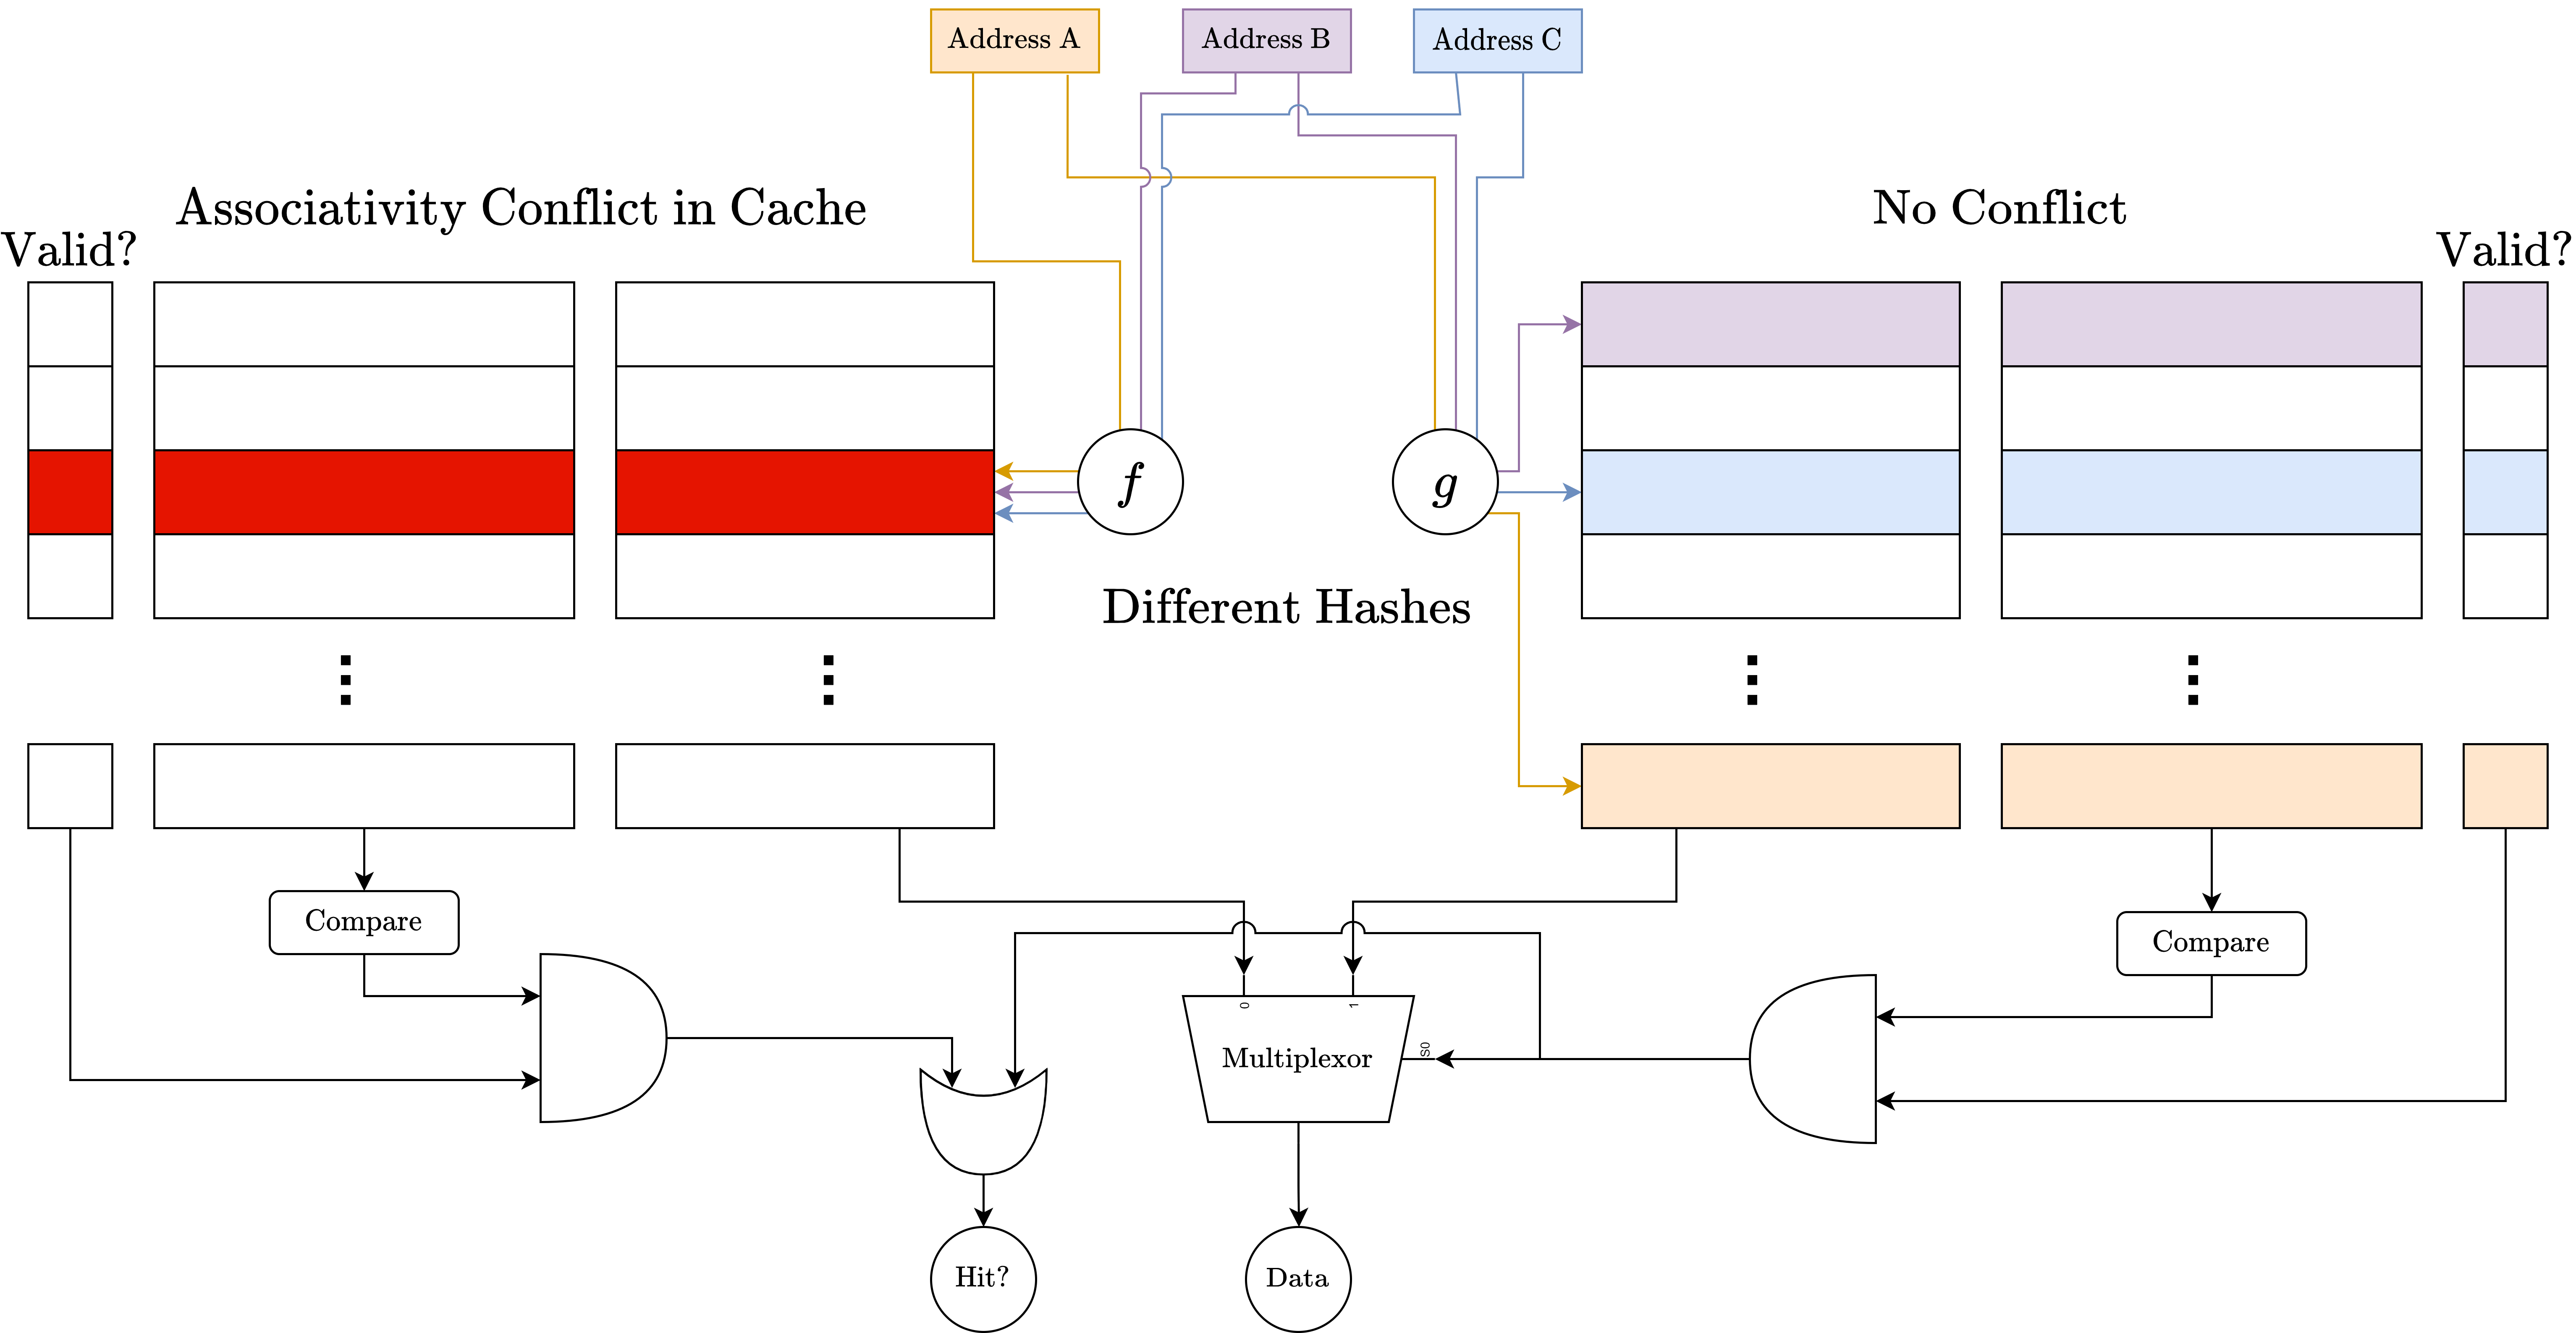
\includegraphics[width=.9\textwidth]{caches/images/skew_associative_cache.drawio.png}
\end{center}
\begin{tabbox}[.6\textwidth]{prosbox}
    \textbf{Associativity Conflicts} & Can reduce associativity conflicts. \\
    \textbf{Reduce Associativity} & Fewer conflicts for a w-way set associativity means the same conflict rate can be achieved with lower associativity (less hardware complexity). \\
    \textbf{More Predictable Average} & e.g with traversing two arrays and a non-skewed cache if we are \textit{"unlucky"} and get an associativity conflict on one element, we will get it on all subsequent. With skewed the next element may not. \\
\end{tabbox}
\begin{tabbox}{consbox}
    \textbf{Some Conflicts} & Its very difficult to write a program free of all conflicts. \\
    \textbf{More Decoders} & Need an address decoder per way/cache rather than a single for all. \\
    \textbf{Hash Latency} & Complex hash increases latency (it is in the critical path). \\
    \textbf{LRU} & Difficult to implement LRU eviction policy (though this is not necessarily a good policy). \\
\end{tabbox}

\subsection{Hardware Prefetching}
When a cache miss occurs, fetch the data (as required), but also pre-buffer the next block in a \textit{stream buffer}.
\begin{itemize}
    \item Prefetched blocks are placed in the cache (would pollute and potentially evict blocks to be used).
    \item Stream buffer checked in parallel with cache.
    \item Can add several prefetch buffers (multi-way stream buffer) to prefetch up $w$-way, fetch to $w$ blocks ahead.
    \item Used in most high performance processors.
\end{itemize}

\begin{tabbox}{prosbox}
    \textbf{Sequential Access} & Can avoid misses when traversing arrays. \\
    \textbf{Cache Untouched} & Can use any type of cache design with this - an addition. \\
\end{tabbox}

\begin{tabbox}[.7\textwidth]{consbox}
    \textbf{Memory Bandwidth} & Need extra bandwidth to transfer block selected (cache miss) and block for pre-fetch. \\
\end{tabbox}

\begin{sidenotebox}{Decoupled Access-Execute}
    Decouple the processor into an access and execution sides.
\begin{itemize}
    \item Access side fetches data to provide to the execute side.
    \item Execute side takes data from access and runs arithmetic instructions on it.
    \item Access side can be far ahead of execute, streaming the required data to it at close to memory bandwidth.
\end{itemize}
\end{sidenotebox}

\section{Miss Rate Reduction Using Software}
\subsection{Software Prefetching}
Many modern processors provide prefetching instructions.
\begin{itemize}
    \item Rarely needed - hardware prefetching is good!
    \item Useful on simpler processors with less or no hardware prefetching.
    \item Care required to prevent unwanted side effects.
    \item Prefetch instructions may target addresses that result in a page fault/protection violation (here they silently fail).
\end{itemize}

\subsection{Reducing Instruction Cache Misses}
Associativity conflicts can occur in the instruction cache.
\begin{itemize}
    \item We want to avoid hot loops calling functions who's code have an associativity conflict with eachother.
    \item By using the caller graph, with each loop labelled, we can determine how to pack subroutines into the program binary to avoid associativity conflicts.
    \item Needs to consider the entire program, and the layout of all subroutines so must be done at link-time.
\end{itemize}


\subsection{Storage Layout \& Iteration Space Transformations}
\begin{center}
    \begin{tabular}{l p{.7\textwidth}}
        \textbf{Merging Arrays} & Improve spatial locality by merging two arrays into a single array of compound elements (i.e a zip). (Struct of Arrays vs Array of Structs) \\
        \textbf{Multidimensional Array Permutation} & Match array layout to traversal order. \\
        \textbf{Loop Interchange} & Change nesting of loops to access data in order stored in memory. \\
        \textbf{Loop Fusion} & Combine independent loops that have the looping behaviour (e.g bounds) and overlapping variables. Sometimes this can then enable \textit{Array Contraction}, where some array can be replaced by a scalar value. \\
        \textbf{Blocking} & Improve temporal locality by accessing cache line sized blocks of data repeatedly instead of accessing columns or rows. \\
    \end{tabular}
\end{center}

\begin{definitionbox}{Morton Ordering}
    A traversal order for blocks.
    \begin{itemize}
        \item Split blocks into four.
        \item Traverse four blocks in $Z$ shape, recursively.
        \item A texture caching layout used in some GPUs.
    \end{itemize}
    \begin{minted}{Haskell}
data QuadTree a = Single a | 
  Quad { 
    topLeft :: QuadTree a, topRight :: QuadTree a, 
    bottomLeft :: QuadTree a, bottomRight :: QuadTree a
  }

{-
 A----->B
        |
 -------
 |
 C----->D
-}

morton :: (a -> b) -> (b -> b -> b -> b -> b) -> QuadTree a -> b
morton fun collect (Quad {tL, tR, bL, br}) 
  = collect (morton' tL) (morton' tR) (morton' bL) (morton' bR) 
  where
    morton' :: QuadTree a -> b
    morton' = morton fun collect
morton fun _ (Single s) = fun s
    \end{minted}
\end{definitionbox}

\section{Miss Penalty Reduction}
\lectlink{https://imperial.cloud.panopto.eu/Panopto/Pages/Viewer.aspx?id=e8fc5064-49d4-45a4-bb1f-af2a01113c4d}{Chapter 3 - Part 3: Reducing Miss Penalty}

\subsection{Write Buffers}
\begin{minipage}{.4\textwidth}
    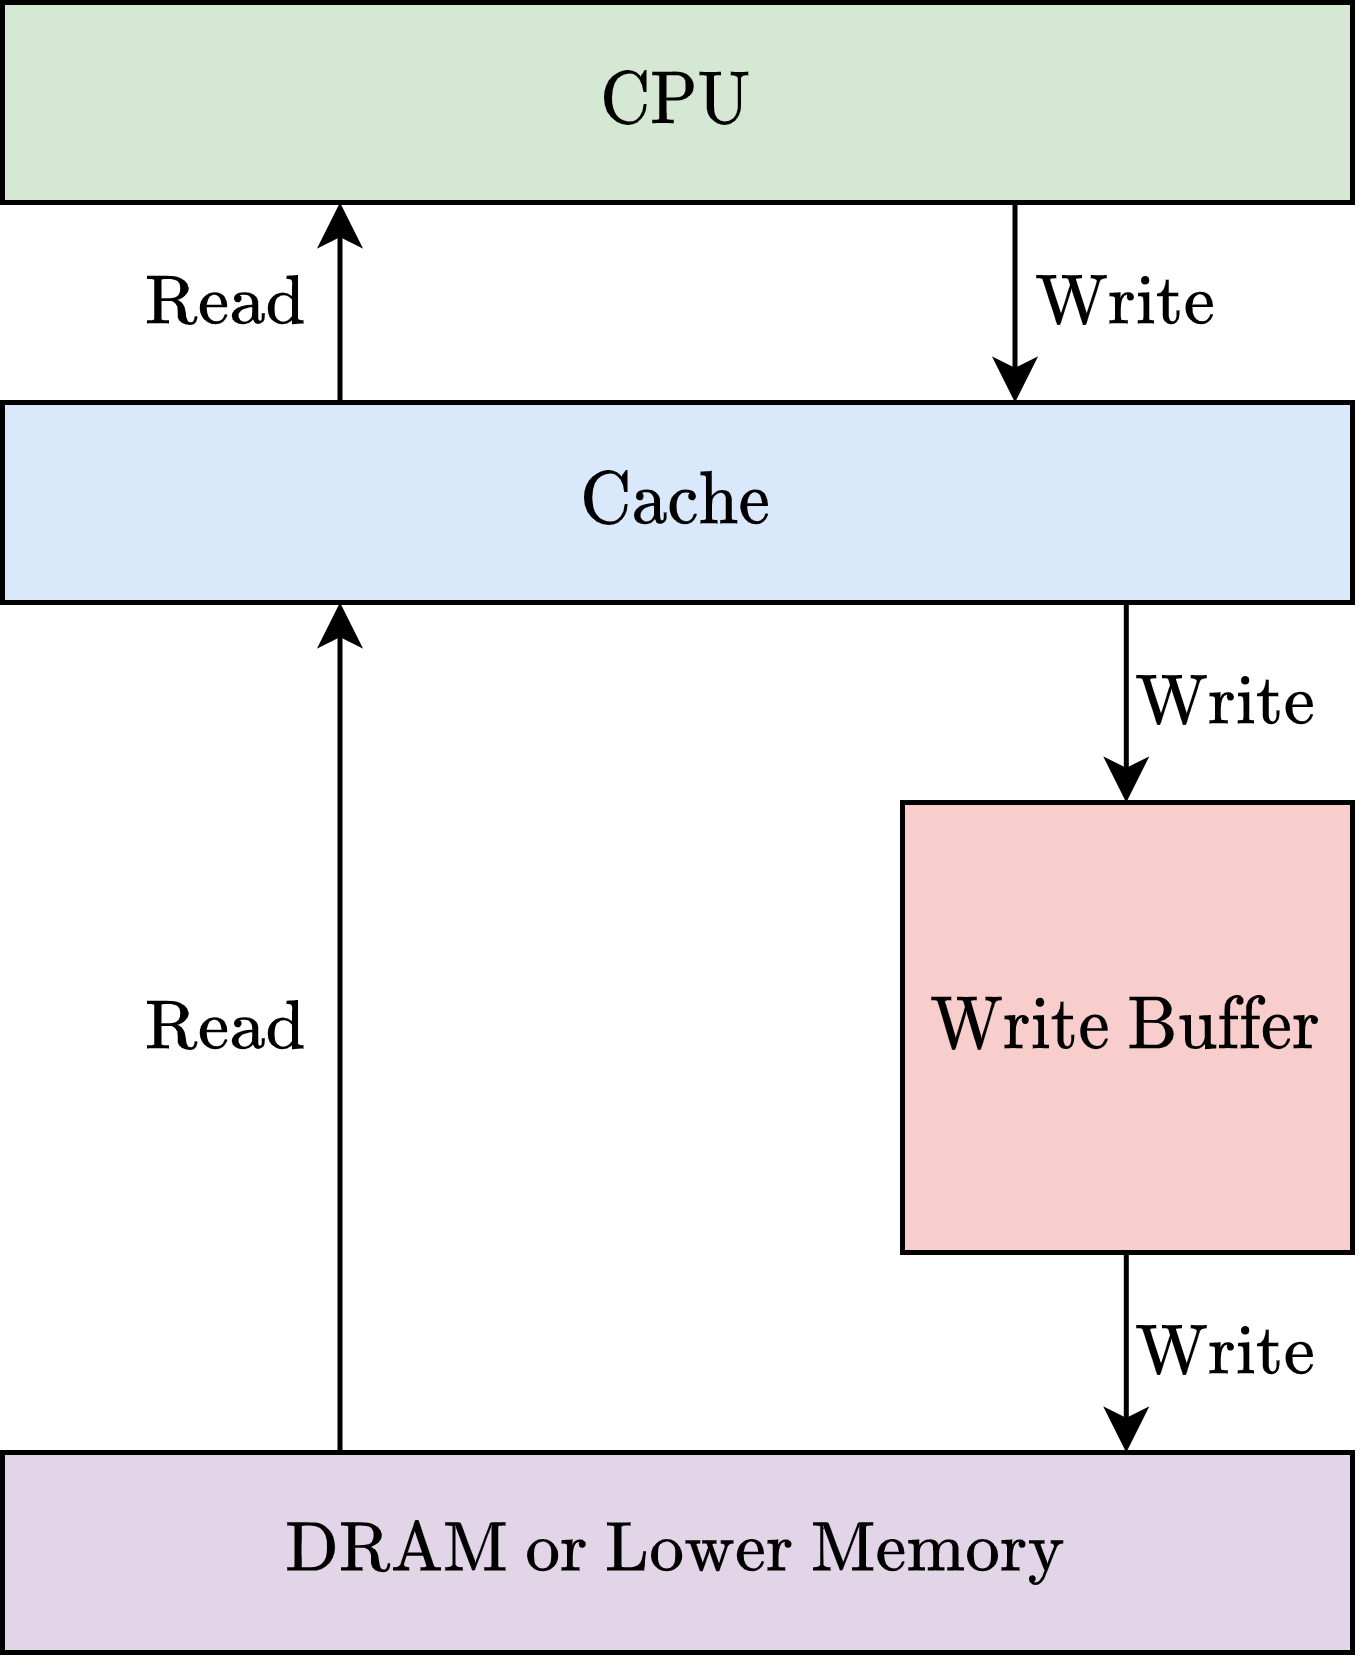
\includegraphics[width=.9\textwidth]{caches/images/write_buffer.drawio.png}
\end{minipage}
\begin{minipage}{.6\textwidth}
    \begin{itemize}
        \item RAW conflict on main memory reads when the location has a write in the write buffer.
        \item One solution is to wait until the write buffer is empty before reading, however this increases the read cache miss penalty
        \item A better solution is to check the write buffer on every memory read, if present in the buffer, take the value from there, else go to memory. 
    \end{itemize}

    With write back we can reduce the stall for a read-miss that evicts a dirty cache line by:
    \begin{enumerate}
        \item Read miss on cache, evict dirty block.
        \item Write dirty block to write buffer (fast).
        \item Start read, CPU can resume/end stall when read is complete.
        \item After read, write from write buffer to memory.
    \end{enumerate}
\end{minipage}
\vspace{5mm}

A cache is structured in terms of lines, hence the eviction of a cache entry means an entire line must be written back to memory.
\begin{itemize}
    \item Larger memory writes require more time, or more expensive/wider buses.
    \item The write buffer needs to be large enough to store multiple lines being evicted. Small write buffer will lead to stalls when full.
\end{itemize}

\begin{center}
    \begin{tabular}{p{.25\textwidth} p{.75\textwidth}}
        \textbf{Coalescing Write Buffers} & Adjacent writes are merged into a single entry in the write buffer. This is especially important in write-through caches. \\
        \textbf{Dependency Checks} & Use comparators to check load addresses against pending stores. On a match a dependency is present, so the load must be stalled (other instructions can run). \\
        \textbf{Load Forwarding} & If a store and load match address, forward the data to the load. \\
    \end{tabular}
\end{center}

\subsection{Early Restart}
\begin{definitionbox}{Sectored Cache Lines}
    A cache line can be divided into sectors.
    \begin{itemize}
        \item Each has its own validity bit, potentially dirty bit also.
        \item Cache allocated in units of cache lines
        \item Data delivered to cache in units of sectors.
        \item Sectors can be fetched in any order, potentially even remaining invalid until requested.
    \end{itemize}
\end{definitionbox}
During a read-miss induced stall, the processor can restart as soon as the requested word arrives.
\begin{center}
    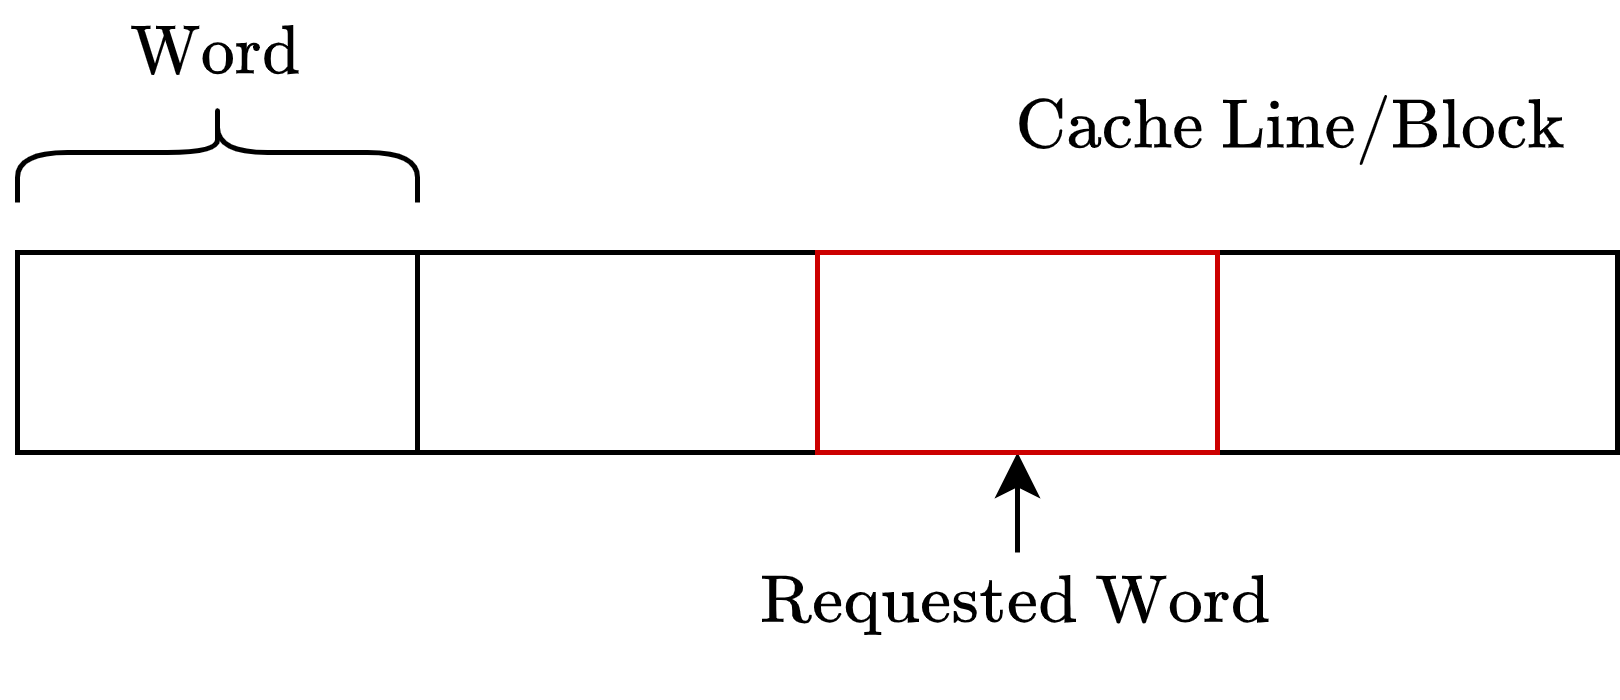
\includegraphics[width=.7\textwidth]{caches/images/cache_block_critical_word.drawio.png}
\end{center}
A cache line consists of many words, when loading a line into cache following a read-miss, we can restart the CPU as soon as the requested word is present.
\begin{center}
    \begin{tabular}{p{.3\textwidth} p{.7\textwidth}}
        \textbf{Early Restart} & As soon as the requested word arrives, send to the CPU and end stall/restart. \\
        \textbf{Critical Word First} & Request the word on which the read-miss occurred from memory first. \\
    \end{tabular}
\end{center}
\begin{tabbox}{consbox}
    \textbf{Complexity} & Sectoring and ordering reads increase hardware complexity. Must be careful for edge cases (e.g read-miss on cache entry that is currently in the process of being loaded). \\
\end{tabbox}

\subsection{Non-Blocking Cache}
\begin{definitionbox}{Non-Blocking / Lockup-free Cache}
    Allows data cache to continue to supply hits for other locations, during a cache miss.
    \begin{itemize}
        \item Requires full/empty bits on registers, and out-of-order execution.
        \item Requires multi-bank memories
    \end{itemize}
\end{definitionbox}

\begin{tabbox}{prosbox}
    \textbf{Hit Under Miss} & Effective miss penalty reduced as useful work is completed during a miss. \\
    \textbf{miss under miss} & Misses are overlapped to reduce effective penalty. \\
\end{tabbox}
\begin{tabbox}{consbox}
    \textbf{Cache Controller} & Needs to support multiple outstanding memory accesses to support \textit{miss-under-miss}. \\
    \textbf{Complexity} & Requires extra hardware (e.g multiple memory banks), and complexities of out of order execution. \\
    \textbf{Fences} & Hit under miss allows for load to be services out of order, hence a fence/barrier instruction must be available to prevent this when required. \\
\end{tabbox}

With In-Order pipeline processors, it is possible to implement some of this functionality by effectively making memory accesses out of order only.
\begin{itemize}
    \item Freeze pipeline in Mem stage, but continue the rest. 
    \item Use full/empty bits on registers, and a MSHR (Miss Status/Handle Registers) queue where each entry tracks the status of an outstanding memory request, a register may be marked as \textit{empty} from a load, it will only stall if still empty when another instruction uses the register, at the decode stage.
    \item This is a popular approach with in-order superscalar processors.
\end{itemize}


\subsection{Multiple Cache Levels}
\[\begin{split}
    AMAT & = \text{Hit Time}_{L1} + \text{Local Miss Rate}_{L1} \times \text{Miss Penalty}_{L1} \\
    \text{Miss Penalty}_{L1} & = \text{Hit Time}_{L2} + \text{Local Miss Rate}_{L2} \times \text{Miss Penalty}_{L2} \\
    & \text{Can continue recursively for }L3, L4 \text{ etc\dots} \\
\end{split}\]
\begin{tcbraster}[raster columns=2, raster equal height]
    \begin{definitionbox}{Local Miss Rate}
        \[\cfrac{\text{Misses for this Cache}}{\text{Accesses to this Cache}}\]
        Misses in a given cache, divided by the total number of memory accesses to the cache.
        \begin{itemize}
            \item Relevant as a cache may not be accessed often, if the cache a level higher has a high hit rate.
        \end{itemize}
    \end{definitionbox}
    \begin{definitionbox}{Global Miss Rate}
        \[\cfrac{\text{Misses for this Cache}}{\text{Total Memory Accesses}}\]
        Misses in a given cache, divided by the total number of memory accesses.
    \end{definitionbox}
\end{tcbraster}

\begin{definitionbox}{Multilevel Inclusion}
    Where lower caches contain all entries in the higher caches.
    \[d \in L1 \Rightarrow d \in L2 \Rightarrow d \in L3\]
\end{definitionbox}
\begin{itemize}
    \item Inclusion strategy affects placement of data, and hence cache controls on coherence, search (should lower caches be checked?) etc.
    \item Can use the L2 cache to filter coherence protocol invalidations. If not in L2, no need to check L1, and hence no need to impact bandwidth to L1.
    \item L3 / LLC (Last Level Cache) often managed as a victim cache, only allocated when data is displaced from L2.
\end{itemize}

\section{Hit Time Reduction}
\lectlink{https://imperial.cloud.panopto.eu/Panopto/Pages/Viewer.aspx?id=1f4afa53-8330-4f04-af28-af2a01118535}{Chapter 4 - Part 4: Hit Time Reduction and Address Translation}

\subsection{Parallel Cache Access}
When attempting to issue multiple instructions per cycle, parallel accesses to the cache are required.
\begin{center}
    \begin{tabular}{p{.2\textwidth} p{.8\textwidth}}
        \textbf{Multiple Banks} & Divide the cache into several banks, with addresses mapped to banks (e.g using low order bits, or a hash function). Accesses to different banks can occur in parallel. \\
        \textbf{Duplicate the Cache} & By using multiple copies of the same cache, each can be accessed separately. \\
        \textbf{Multi-ported RAM} & Add another wordline per row, and another bitline per column to allow multiple accesses to the RAM at the same time, cache uses this multiported RAM. This is effectively duplicating the cache, but sharing the flipflops between caches. \\
    \end{tabular}
\end{center}


\subsection{Address Translation}
\begin{center}
    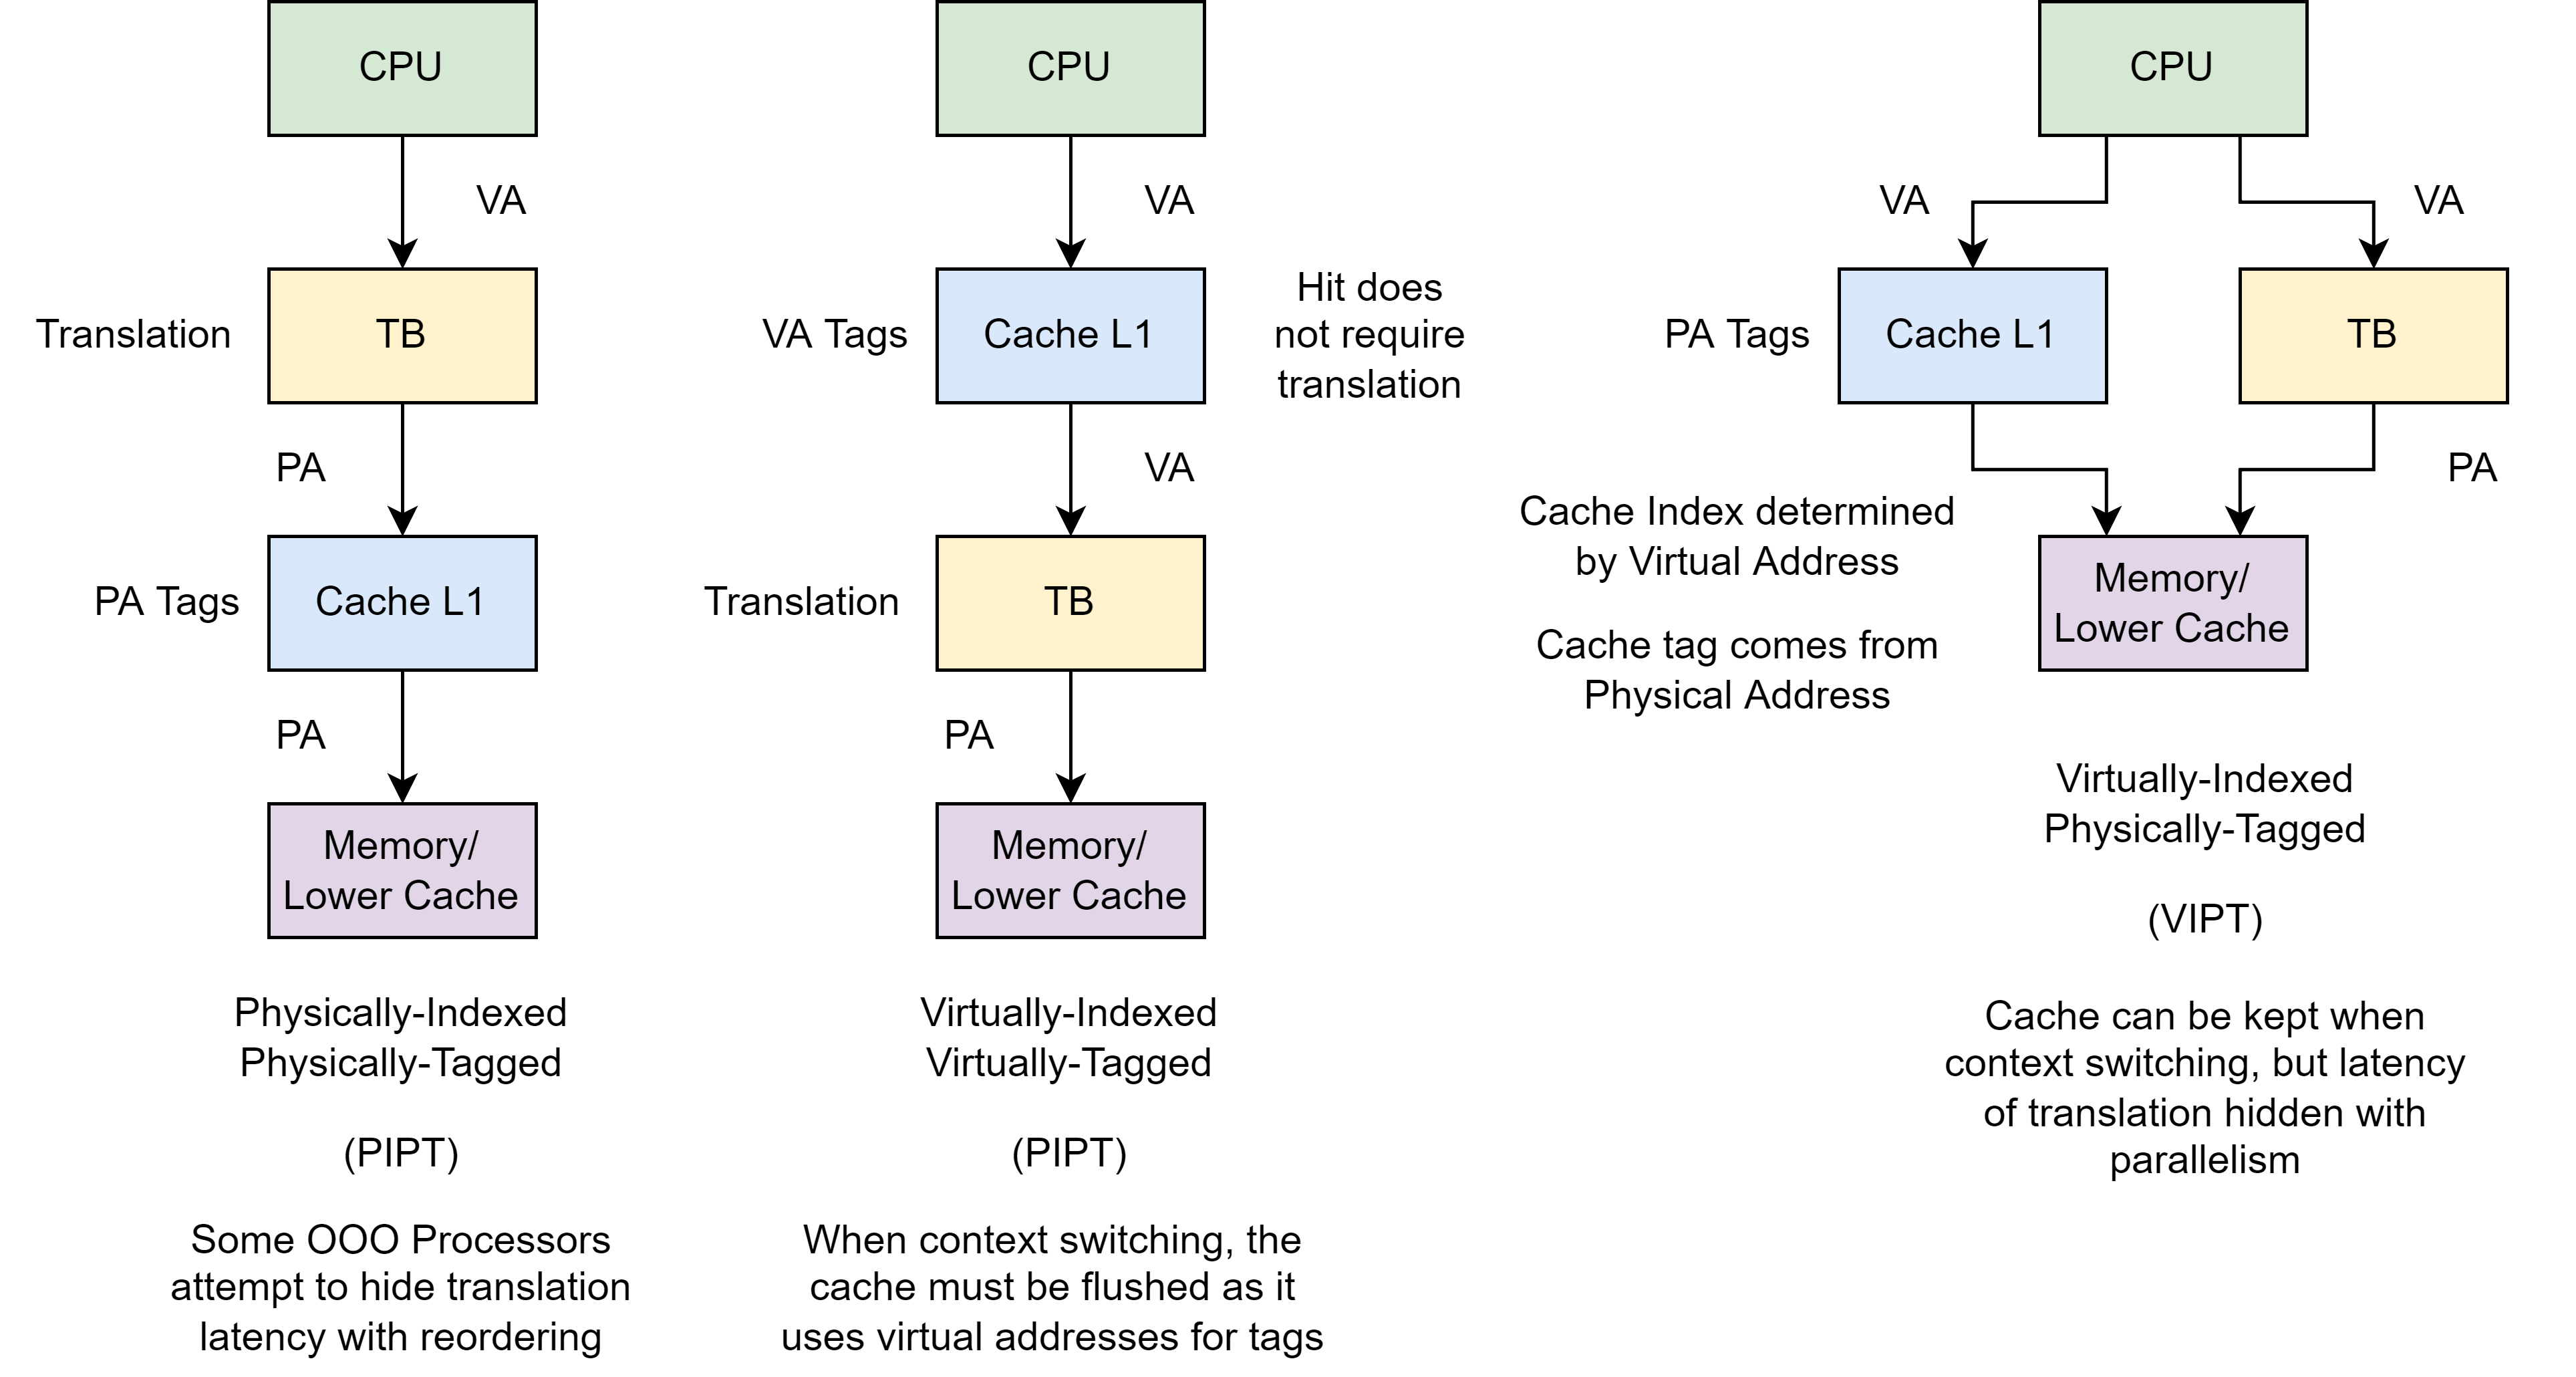
\includegraphics[width=\textwidth]{caches/images/address_translation.drawio.png}
\end{center}
\begin{tcbraster}[raster columns=2,raster equal height]
    \begin{definitionbox}{Homonyms}
        \centerline{\textit{Same sound, different meaning}}
        The same virtual address can point to different physical locations, in the context of different processes.
        \begin{itemize}
            \item A virtually indexed cache, as the tags are compared to determine hit/miss, we must flush the cache.
            \item In a TLB, where the cache is necessarily virtually tagged \& indexed, a flush must occur, unless some process identifier is included in the tag (e.g ASID - Address Space ID).
        \end{itemize}
    \end{definitionbox}
    \begin{definitionbox}{Synonyms}
        \centerline{\textit{Same meaning, different sound}}
        \begin{itemize}
            \item Multiple virtual addresses point to the same physical.
            \item In a virtually indexed cache multiple addresses may map to the same page.
            \item Updates to one cached copy must be reflected in the others (shared pages)
        \end{itemize}
    \end{definitionbox}
\end{tcbraster}

\subsubsection{Faster Cache Hits by Avoiding Translation}
\begin{center}
    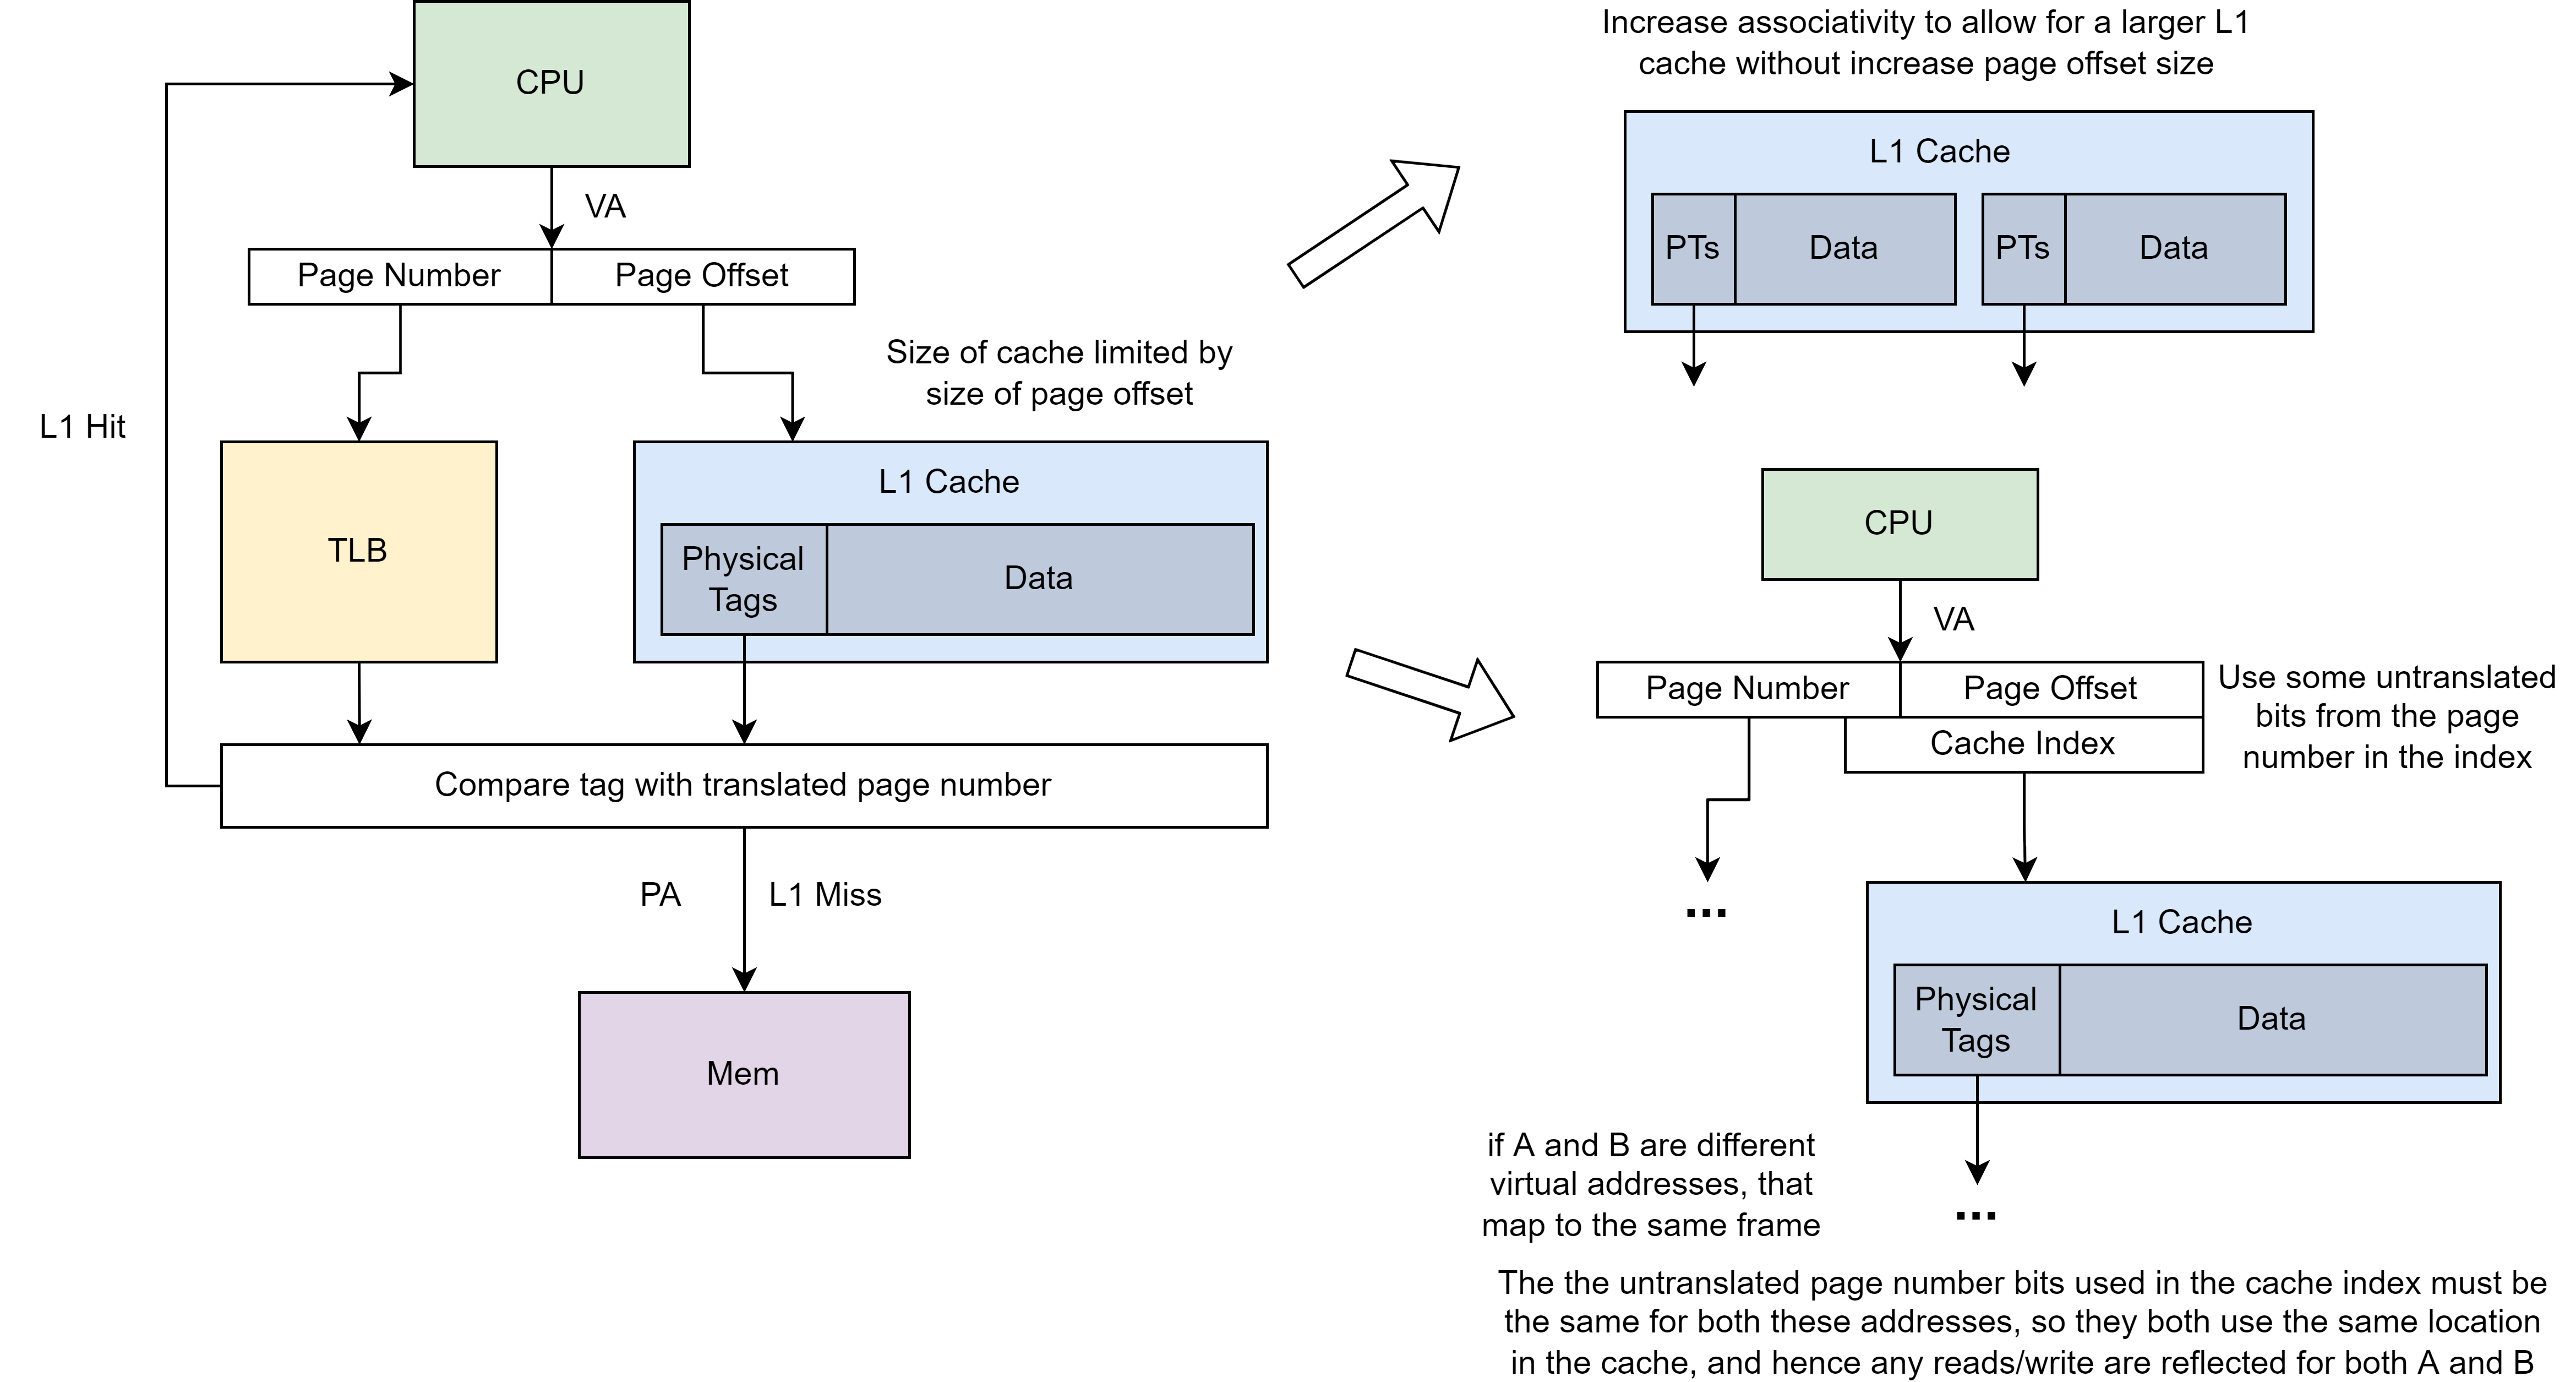
\includegraphics[width=\textwidth]{caches/images/fast_cache_hit_index_offset_bits.drawio.png}
\end{center}
\begin{sidenotebox}{Linux MMap}
    \mintinline{C}{mmap} in linux does not specify the address in order to allow the operating system to determine this. This allows the OS to perform system specific tricks such as ensuring the page number bits in the cache index are identical for virtual addresses mapped to the same frame.
\end{sidenotebox}
The L2 cache makes use of physical addresses, and hence relies on the virtual-to-physical mapping provided by the OS.
\begin{itemize}
    \item The OS may choose mappings that result in associativity conflicts in the L2 cache.
    \item This means that different instances of the same program, with the same computation can have different performance, as the OS may assign frames such that an associativity conflict occurs.
\end{itemize}
Operating systems can also use different page sizes.
\begin{itemize}
    \item large pages require smaller page tables, and use fewer TLB entries, which increases the hit rate for the TLB.
    \item Requires support in hardware for multiple page sizes.
\end{itemize}
